Chapter \ref{ch:approach} has formalized the problem and put forward a novel framework for finding useful words, consisting of two major functionalities:
Vocabulary list generation, and vocabulary list evaluation.
The list evaluation approach, described in Section \ref{sec:experimental-setup-with-ai}, utilizes the performance of an AI model on an NLP task with a context-specific corpus as input as a proxy metric for language ability, in order to estimate how efficiently the vocabulary list may help a human language learner acquire competency.
The list generation approach, proposed in Section \ref{sec:list-generation}, additionally uses Explainable AI as a tool for analyzing the interaction of the AI model with the corpus to compile vocabulary lists that approach maximal efficiency.

In this chapter, we describe our implementation, especially of the list generation approach.
This is because the list evaluation method is used in Chapter \ref{ch:evaluation} as one among several metrics for evaluating the efficiency of vocabulary lists generated by the implementation in this chapter.
However, the evaluation with our approach uses the same AI models and Corpora as the list generation approach.

We first discuss the implementation of the list generation approach from a system design perspective in Section\ref{sec:data-pipeline}, describing how we generate lists of vocabulary, without elaborating on the interdependencies that arise between concrete NLP tasks, corpora, and XAI methods.
The choice of those three components in the system is then argued in the following sections, each of which features a section where we discuss desiderata of the specific component on the basis of our aim as stated in Section \ref{sec:formal-problem-statement}, followed by the selection of concrete components.
Finally, we return to the holistic perspective in Section \ref{sec:implementation-final}, where we present the complete implementation with all individual components integrated.

\section{Data Pipeline} \label{sec:data-pipeline}

This section gives a top-level overview of our implementation for the list generation approach described in Chapter \ref{ch:evaluation}.
As mentioned before, the main components of this approach are:

\begin{itemize}
	\item An AI model, used as a test subject.
	\item An NLP task, the score in which is used as a proxy metric for the language ability of the test subject.
	\item A context-specific corpus, to model a language context.
	\item An XAI method, which analyzes the interaction of the AI model with the corpus to determine word utilities.
	\item If the XAI method allows: A tokenizer, determining the words to be analyzed.
\end{itemize}

Thus, the implementation of the approach mainly consists of determining how exactly these components interact, as well as deciding which model, XAI method, and corpus, is used.
The interaction of these components can be seen in pseudocode in Algorithm \ref{alg:efficient-list-generation}.

\begin{algorithm}
\caption{Efficient List Generation.}
\label{alg:efficient-list-generation}
\begin{algorithmic}[1]
\Require corpus, model, xai\_method
\State Initialize $line\_word\_utilities$ with empty list

\For{each $line$ in $corpus$}
    \State $word\_utilities\_for\_this\_line \gets$ xai\_method$(model, line)$
    \State Append $word\_utilities\_for\_this\_line$ to $line\_word\_utilities$
\EndFor

\State $corpus\_word\_utilities \gets$ aggregate($line\_word\_utilities$)
% \State $corpus\_word\_utilities\_scores$ $\gets$\newline
% aggregate\_word\_utilities($line\_word\_utilities\_scores$)

\State $voc\_list \gets$ words ordered by $corpus\_word\_utilities$

\State \Return $voc\_list$
\end{algorithmic}
\end{algorithm}


The XAI method outputs the importance attributions in the form of one number for each unique word in each input line.
The results are aggregated by taking the sum across all lines in the corpus, resulting in a list of word-utility pairs, which reflect the estimated utility of the word with respect to the entire corpus.
To make a vocabulary list from these words, we simply order the words by their estimated corpus utility in descending order.

With this basic structure established, the following sections address the selection of individual components.
Due to the interdependencies between certain components, not all are presented in separate sections.
The NLP task performed depends on the AI model that we use, as most AI models are trained on only one task.
Therefore, the choice of AI model is discussed together with the NLP task in the next section.

\section{NLP Tasks and AI Models}
Our approaches for list efficiency evaluation and for efficient list generation use an AI model with an NLP task to simulate a test subject performing a language exam.
Because of this, the AI model and task chosen are a crucial component of these approaches, and their selection is among the most important in the implementation.
The NLP tasks we choose also influence what corpora we can use for their execution:
The task of next sentence prediction requires contiguous texts as input data, necessitating input corpora containing whole documents, not just individual sentences.

This section first puts forward criteria for selecting NLP tasks in Section \ref{sec:nlp-tasks-desiderata} for word utility evaluation.
% After this, we use these criteria to select a few NLP tasks as appropriate in Section \ref{sec:nlp-tasks-selection}.
We then discuss potential candidate NLP tasks, and discuss how appropriate they are for our approach.
In the final selection, we decide on two tasks which, in the estimation of the author of this work, are suitable for our word utility evaluation approach, namely \textit{next sentence prediction} and \textit{sentence embedding}.
These NLP tasks we choose dictate the format of our input data, i.e., the corpora we can use.
Therefore, the selection of corpora is discussed after the choice of NLP is finalized.

\subsection{Desiderata} \label{sec:nlp-tasks-desiderata}

This section puts forward four criteria for selecting NLP tasks for word utility evaluation, arising from our underlying goal of using the task as a proxy for real language interaction of a human being:
The availability of many multilingual AI models and corpora usable as input for the task, generality of the task and ease of evaluation.
These criteria are used in the next section to select concrete tasks for our implementation.

\subsubsection{Model Availability in Many Languages}
The goal of this work is to find approaches to find useful words for the purpose of language learning.
Much research in Natural Language Processing is dedicated to improving NLP performance in English and other high-resource languages such as English, French or Mandarin Chinese \cite{joshiStateFateLinguistic2021}.
This has the consequence that many AI models and other NLP methods achieve high levels of performance only in these languages, and many AI models are only available in English or only a small number of languages \cite{joshiStateFateLinguistic2021}.
However, there are over 7,000 languages in the world \footnote{According to \textit{Ethnologue} (\url{https://www.ethnologue.com/}, last accessed on April 22, 2025)}, and for many of these there exist corpora, or online digital texts which can be used as inputs for our word utility evaluation approach, such as Wikipedia articles, \textit{Open Parallel Corpora}  (OPUS) \footnote{\url{https://opus.nlpl.eu/}}, or \textit{Wortschatz Leipzig} \footnote{\url{https://wortschatz.uni-leipzig.de/}}.
In order to make an implementation with the potential to exploit the linguistic diversity in these resources to the fullest extent, we only consider NLP tasks for which pre-trained models exist which can process a high number of languages.

\subsubsection{Corpus Availability in Many Languages}
The second point of consideration for task selection is \textbf{how much data is available for performing the task}.
Ideally, we would like tasks for which suitable corpora are freely available or can be trivially generated from available corpora.
This is because, with a larger amount of usable data, we not only improve the accuracy of our approach, but also increase the diversity of input data.
Because context-specific language learning is a central motivation of this work, diverse training data is desirable, as it provides a broader range of linguistic contexts to model and from which to identify useful words.

\subsubsection{Generality of Skill Required}
Another important point to consider when selecting an NLP task is \textbf{how general the linguistic skills} are that the task requires:
We use the performance in the NLP task as a proxy metric for the test subject's language ability.
As such, we must ensure that task reflects a general level of semantic understanding, not only a narrow mechanistic skill that can be accomplished by using only a small part of the input.
For this reason, we do not consider tasks such as part-of-speech tagging and text classification appropriate, as they do not reflect skills of language speakers used in everyday life.

\subsubsection{Ease of Evaluation} \label{sec:ease-of-evaluation}
To ensure we can measure task performance, we must also choose a task whose results can be easily compared with each other:
Some tasks are difficult to evaluate objectively, or the evaluation takes an inordinate amount of computation (see Section \ref{sec:text-summarization} on text summarization).
It follows that if we have the freedom to choose NLP tasks whose results can be automatically evaluated with good accuracy, we should choose them.


\subsubsection{Summary of Desiderata}
To summarize our desiderata for NLP tasks:
Our implementation seeks to use NLP tasks for which AI models and Corpora exist in a large number of languages, to make our approach for finding useful vocabulary usable in the greatest number of languages.
We prefer tasks that demonstrate general language understanding over tasks that only require a narrow skill set to perform or that are too technical, because general tasks are expected to align more with human linguistic skills.
Finally, the task must be easily scorable, since the task score is the metric by which we gauge how useful words are.
The next section introduces several candidates, primarily by surveying which tasks are commonly used as pre-training tasks for state-of-the-art language models, as these must fulfill similar requirements to those stated in this section.

\subsection{Survey of Candidate NLP Tasks}
This section introduces several NLP tasks we use in our implementation, as well as some tasks which were not selected.
We first describe the process of how candidate tasks were found, and then go into detail for each candidate as to why it was or was not selected in the following subsections.

Candidates were first compiled by surveying common pre-training tasks which are used in state-of-the-art NLP models:
This is because the purpose of a pre-training task is to endow the AI model with a general understanding of the language, before either using transfer learning to specialize it for a more specific downstream task, or using it before another downstream AI model to pre-process input \cite{jurafskySpeechLanguageProcessing2025a}.
Such tasks must necessarily be general and require general language understanding, since training the model with them is supposed to provide a solid basis for a wide variety of NLP tasks.
Another benefit of using pre-training tasks is that their training is unsupervised, meaning there is no need to manually label data.
Their widespread use in \NLP also means that pre-trained models are widely and freely available.
From this consideration, we select language modeling and next sentence prediction as candidates, but reject language modeling for the reasons below.
In addition to these common pre-training tasks also consider text summarization and sentence embedding, however, because text summarization is difficult to evaluate, reject this task as well.

\subsubsection{Language Modeling}
There generally exist two subtypes of language modeling, namely Causal Language Modeling and Masked Language Modeling \cite{jurafskySpeechLanguageProcessing2025a}.
Causal language modeling describes the task of predicting the text token in a text, given the sequence of previous tokens, and it constitutes the basis of many recent developments in Large Language Models \cite{brownLanguageModelsAre2020} \cite{openaiGPT4TechnicalReport2024}.
Masked language modeling involves filling in missing tokens in a sentence, and is one of the training tasks for the popular BERT models \cite{kentonBertPretrainingDeep2019}, along with next sentence prediction.

While its training data can be trivially generated from corpora and does not pose great challenges in evaluation, we did not consider either type of language modeling an appropriate NLP task for the purpose of finding useful vocabulary.
This is because generating the task's training data already involves removing tokens from the input, resulting in training data with word distributions which do not correspond to language found in real texts.
Another issue arises to the nature of model-agnostic, feature importance attribution XAI methods:
These methods perturb the input to determine which tokens in the input are the most relevant.
However, whether or not a token is appropriate as the next token in a document is sure to change with even slight perturbations:
Consider the sentence:

\begin{quote}
	\textit{The sky is blue.}
\end{quote}

A language model, given the input datum \textit{The sky is}, may be able to predict that \textit{blue} is a probable next word to this sentence.

However, if we mask the --- relatively unimportant --- word  \textit{is} in the sentence to find out if the model's can predict the last word of the sentence even when \textit{is} is missing, we are left with the sentence:

\begin{quote}
	\textit{The sky}
\end{quote}

For this variation, \textit{blue} is no longer an appropriate next word to predict, as this would result in a grammatically incorrect sentence.
This would lead a feature importance attribution method to evaluate \textit{is} as a very important word in the sentence, because its absence leads to a loss of accuracy, despite it being unimportant to the overall meaning of the sentence.
These complications make it difficult to use feature importance attribution methods on language modeling, which is why we decided against the use of this task for our implementation.


\subsubsection{Next Sentence Prediction}
In Next Sentence Prediction (NSP for short), the AI model takes as input two sentences and predicts a probability for the second sentence being the successor of the first sentence in their source text \cite{kentonBertPretrainingDeep2019}.
Input data for this task, including labels, is trivial to generate from document-level corpora, as it merely requires a corpus of sentences that follow from each other, which is easily obtained from Wikipedia articles, film subtitles, or any other continuous text.
As the output of next sentence prediction is one number expressing the predicted probability of the input sentences following each other, its performance is also easy to calculate, using cross-entropy.
While predicting whether two sentences are consecutive may not seem like a transferable skill, it is used as one of two pre-training tasks for BERT models \cite{kentonBertPretrainingDeep2019}, which suggests that using this task in pre-training imbues the model with transferable language skills.
For these reasons, we use the NSP task in our word evaluation approach.


\subsubsection{Text Summarization} \label{sec:text-summarization}
This task involves summarizing a given text, in other words, writing a shorter version of the input text while still conveying as much of the information from the original text as possible \cite{radevIntroductionSpecialIssue2002}.
Summarizing texts accurately would seem to require a high level of understanding of the text, and thus be good choice for testing whether ablating certain words from the text has detrimental effect on the model performance.
Unfortunately, this task is not appropriate for our purposes with respect to our other desiderata, because evaluating the quality of a summary is a very challenging task:
It involves a ground truth summary which is usually manually created, against which another summary is compared.
This already makes the use of this task problematic for low-resource languages (languages for which only few or only small NLP datasets exist), as text summarization datasets are scarce for these \cite{dahanStateFateSummarization2025}.
However, even assuming sufficient data, the comparison of two summaries is difficult:
A standard way of evaluating summaries are ROUGE scores \cite{allahyariTextSummarizationTechniques2017}:

These measure the overlap of n-grams (word sequences) between two texts.
However, it is questionable how well they capture the similarity between texts, because they do not recognize the semantic similarity of synonyms, and a different sentence structure will result in a low ROUGE score even if the actual meaning of the sentences may be very close.
For these reasons, we do not use text summarization in our implementation.

\subsubsection{Sentence Embedding} \label{sec:sentence-embedding}
Sentence embedding takes sentences as inputs and outputs vectors of numbers, which are typically used as inputs for a downstream task such gauging the similarity between two sentences, which can in turn be used to find similar sentences across languages for making training data for translations model \cite{artetxeMassivelyMultilingualSentence2019} \cite{reimersMakingMonolingualSentence2020}.
This approach can be performed on any corpus containing distinct sentences, meaning the corpus does not have to be document-level, and sentences need not be consecutive.

An important characteristic of this task is that it has no ground truth labels, and therefore, when using feature importance attribution XAI methods, we cannot measure differences in performance of the downstream task when the input is perturbed.
Instead, we embed an input sentence in its original form (the baseline embedding), then embed variations of the sentence with some of its words removed, and measure the distance between the baseline embedding and the embedding of each variation.
A large distance between the baseline and the variant embedding where a word has been removed implies that the removed word is useful for understanding the sentence.
We believe these distances are a valid metric for determining how much a word contributes to the meaning of the sentence, as the embedded vector is already a semantic representation of the input.
In our estimation, the ease of evaluation and of finding input data, as well as its generality make sentence embedding an ideal task for word utility evaluation, which is why we use it not only for the generation of vocabulary lists, but also for the evaluation of their efficiency.

\subsection{Choice of Model}
In the previous sections, we have presented two tasks which seem appropriate choices for our vocabulary list generation and evaluation approach, namely, next sentence prediction and sentence embedding.
This section discusses the choice of the AI model used for both of these tasks.
In general, we use models from model families which support many languages, but the concrete models in our implementation are monolingual models, as these have shorter inference times, allowing us to process more data.

\subsubsection{Next Sentence Prediction Model}
As our next sentence prediction model, we use a BERT model \cite{kentonBertPretrainingDeep2019}, as these models have been trained in many languages (over 104 for \texttt{bert-base-multilingual-cased}, the model with the most languages \footnote{\url{https://huggingface.co/google-bert/bert-base-multilingual-cased}}).
As BERT models have the same structure to each other, this makes extending our approach to more languages trivial:
We use the model-specific XAI method of attention (see Section \ref{sec:transformer}) in our pipeline, the implementation of which is dependent on the transformer used, as the attention tensor's dimensions are dictates by variables such as the number of attention heads.
However, for our implementation, we employ the monolingual English model \texttt{bert-base-uncased} \footnote{\url{https://huggingface.co/google-bert/bert-base-uncased}} for its smaller size (110M parameters instead of 170M for \texttt{bert-base-multilingual-cased}) and shorter inference time.


\subsubsection{Sentence Embedding Model}
For the sentence embedding task, there are two model families that appear as suitable candidates for our implementation:
\textit{LASER} embedding models \cite{artetxeMassivelyMultilingualSentence2019}, developed by Meta, and \textit{Sentence Transformers} a.k.a. \textit{sBert} \cite{reimersMakingMonolingualSentence2020}, developed chiefly by the University of Darmstadt.
Both of these solutions have set as their aims the embedding of sentence of as many languages as possible, giving special considerations to low-resource languages. 

While the latest \textit{LASER} embedding model is more recent and claims to outperform previous models, its implementation requires a Unix environment to work, which presented compatibility issues with our Windows-based development setup \footnote{\url{https://github.com/facebookresearch/LASER}}.
Additionally, to the best of our knowledge, the models are not available on the \textit{HuggingFace} \footnote{\url{https://huggingface.co/}} platform, meaning their use would have necessitated various changes in our implementation due the different interface.
For this reason, we use the models from the \texttt{sentence-transformers} package.
While the models are available in their dedicated Python package \url{https://www.sbert.net/}, these do not allow for the output of attention values, which is why we load the Sentence Transformer model from HuggingFace directly.
This necessitates an additional post-processing step, but the code is available on the model website.
The model we use is \footnote{\url{https://huggingface.co/sentence-transformers/all-MiniLM-L6-v2}}.
This model is a monolingual English model, however again, it is much more lightweight than the multilingual Sentence Transformer models.



\subsection{Summary}
We have put forth desiderata for the NLP tasks to make our approach to vocabulary list generation and evaluation accurate, as well as applicable to many languages and language contexts.
As a result of these desiderata, we have chosen the two tasks of next sentence prediction and sentence embedding, for the general language skill they require, because they are easy to evaluate automatically, and because input data for them is trivial to acquire in many languages.
The next section discusses the choice of corpora which are used as input data for these tasks.


% \subsection{Use of Selected Tasks in this Work}
% \subsection{Next Sentence Prediction}
%
% \begin{description}
% 	\item[LASER] \cite{artetxeMassivelyMultilingualSentence2019}
% 	\item[BERT] \cite{reimersMakingMonolingualSentence2020}
% \end{description}
%
% \subsubsection{Choice of Model}
% \subsubsection{Data Required}
%
% Requires a corpus that contains consecutive sentences.
% Furthermore, NSP typically predicts whether two sentences follow each other in a document, not a dialogue (see the data on BERT training \cite{kentonBertPretrainingDeep2019}).
% This excludes movie subtitles from the possible corpora for this task.
%
%
% \subsection{Sentence Embedding}
% \subsubsection{Choice of Model}
% \subsubsection{Data Required}



\section{Corpora}
In the previous section, we put forth criteria for which NLP tasks should be used in our word utility evaluation approach, and decided on the two tasks of next sentence prediction and sentence embedding.
Having decided on these, we now require data, i.e., corpora, as inputs for the tasks.
Which corpora we use is another important decision, as these serve the purpose of modeling the language contexts in which the language learner is striving to achieve proficiency.
This section therefore first states our general selection criteria for corpora.
We then introduce publicly available corpora which are suitable for our evaluation approach, and conclude by choosing Wikipedia and OPUS subtitle data as inputs for the NLP tasks.
For the background corpus used to calculate the inverse document frequency in TD-IDF, we use a corpus from the \textit{Oscar} project (see Section \ref{sec:oscar}).

\subsection{Desiderata}
This section puts forward our general criteria for corpus selection, following from our overarching goal of using the model to model linguistic contexts for the purpose of language learning.
In short, we use corpora which are available in many languages, allow for the modeling of different linguistic contexts, and consist of continuous texts to provide data for the NLP tasks.

\subsubsection{Document-Level Corpus} \label{sec:document-level-corpus}
The first desideratum for our corpora stems from our choice to use next sentence prediction as one of our NLP tasks:
As next sentence prediction predicts whether one sentence is likely the continuation of another, it requires contiguous sentences pairs to work.
To generate these pairs, we must use (at least some) corpora featuring continuous tests, not only individual sentences.
This presents a challenge, as many corpora which are compiled from Web Crawls, such as the corpora from \textit{Wortschatz Leipzig} \footnote{\url{https://wortschatz.uni-leipzig.de/}}, contain only scrambled, single lines to avoid copyright infringements (single sentences cannot be put under copyright in certain states \cite{goldhahnBuildingLargeMonolingual2012}).
However, Wikipedia contains articles on many different topics which do not underlie strict copyright license (see Section \ref{sec:wikipedia}), which makes it appropriate for our purposes.

\subsubsection{Free Availability in Many Languages}
In Section \ref{sec:nlp-tasks-desiderata} we put forward reasons for why freely available AI models which can handle a diverse pool of languages are desirable for our undertaking.
By the same token, we also prefer corpora which are publicly available in many languages over corpora which only include data in one language.
While a monolingual corpus is not inferior to a multilingual one, its use necessitates that the user manually compile many corpora if a multilingual implementation is to be achieved.

\subsubsection{Closeness to Linguistic Contexts Desired by Language Learners}
As mentioned before, the corpus in our word utility evaluation approach serves the purpose of modeling a linguistic context, and this linguistic context should reflect some set of situations that a language learner is likely to find themselves in.
Typical situations would include reading the news, reading literature or watching movies in their target language.
As such, corpora which are close to the materials which language learners are likely to engage with are desirable, since their use makes the AI model's performance on the task more reflective of skills that a language learner would like to acquire.

\subsubsection{Divisibility of Corpus into more Specific Corpora}
Not only the relevance of the entire corpus's linguistic context is important:
Some corpora enable us to further split them up into smaller corpora with more specific language contexts.
For instance, while we can use a corpus such as \textit{Wikipedia} as a whole, the structure of Wikipedia enables us to group articles by the category they belong to (politics/sports etc.), or even use single articles, to find more specific contexts.
Such corpora are especially efficient for generating multiple contexts, hence we make use of such corpora.


\subsubsection{Rejected Corpora} \label{sec:rejected-corpora}
This section briefly describes two corpora which may appear to be useful for our word utility evaluation approach, but which we do not believe are appropriate.

\paragraph{Common Crawl:}
A common choice for training large language models is the \textit{Common Crawl} dataset \footnote{\url{https://commoncrawl.org/}}.
Its size and diversity could make it useful either as a corpus for modeling a "surfing the web" linguistic context, or as a background corpus to calculate TF-IDF on other corpora.
However, we reject both uses of it:
Firstly, in its raw form, it takes the form of HTML code and includes much boilerplate content such as cookie requests, necessitating much preprocessing.
More importantly, speaking against its use as a context-modeling corpus, its data is not grouped by topic or language, which means we cannot trivially generate more topic-specific corpora from it, nor utilize it for different languages without a significant amount of pre-processing.

\paragraph{Wortschatz Leipzig:}
\textit{Wortschatz Leipzig} \footnote{\url{https://wortschatz.uni-leipzig.de/}} provides corpora in more than 100 languages, and groups these by their source such as "News", "Wikipedia", and "Web".
We also rejected the Wortschatz Leipzig Corpora because, while these corpora are stripped of any HTML code, they are composed of single lines collected from websites, rather than whole documents.
Although we considered using one of the "Web" corpora for calculating inverse document frequency for the TF-IDF metric, the original paper for the Wortschatz corpus also states that political content was utilized in bootstrapping the web searches for data gathering, including the \textit{Universal Declaration of Human Rights} and the Jehova's Witnesses magazine \textit{Watchtower} \footnote{Previously available at \url{watchtower.org}}, which may lead to a respective bias in the final corpus \cite{goldhahnBuildingLargeMonolingual2012}.
Thus, we did not use \textit{Wortschatz} corpora as a background corpus, either.

\subsection{TF-IDF Background Corpus: Oscar} \label{sec:oscar}
For the implementation of TF-IDF, we require a generic background corpus to normalize raw word frequencies found in context-specific corpora (that is, to calculate the IDF part of TF-IDF).
For this purpose, corpora crawled from the internet offer themselves as an attractive option, as web content is diverse in that it encompassed both formal and informal content on many different topics.

We reject the Common Crawl and Wortschatz Leipzig datasets for the reasons already stated in Section \ref{sec:rejected-corpora}.
Instead, we use a corpus from the \textit{Oscar} project \footnote{\url{https://oscar-project.github.io/}} as a background corpus:
Each \textit{Oscar} corpus is a cleaned-up version of a \textit{Common Crawl} dataset, on which preprocessing steps such as HTML stripping and removal of boilerplate content have already been performed.
It consists of (whole) web pages, and most importantly, its content is language-tagged, covering more than 150 languages in total.
There exist many versions of the Oscar dataset, but for this work, the \textit{mOscar} \cite{futeralMOSCARLargescaleMultilingual2024} corpus from 2024 was chosen, both for its recency and coverage of many languages.
Due to its vast size, we did not use the entire corpus, but a random sample of 53,179 documents from this dataset to calculate inverse document frequency.

\subsection{Wikipedia} \label{sec:wikipedia}
Our primary source for corpora are articles from Wikipedia \footnote{\url{https://www.wikipedia.org/}}.
Wikipedia is a valuable resource for several reasons:
It contains a vast number of articles, and about a diverse set of topics.
Wikipedia articles are assigned article categories describing their topic, such as "20th century American male actors".
This means we do not have to group articles into topics ourselves, enabling us to trivially create corpora that model linguistic contexts more general than a single article, but more specific than Wikipedia as a whole.
The characteristics of the article category system on Wikipedia are discussed below.

Wikipedia's articles are licensed under the Creative Commons Attribution-ShareAlike 4.0 International License (\textit{CC BY-SA}).
Because of this, Wikipedia can provide dumps of its entire article database ready for download, with the articles in continuous form and with category metadata attached to them \footnote{Available for download at \url{https://dumps.wikimedia.org/}}.
This enables us to use the articles as a source for the next sentence prediction NLP task.

While Wikipedia offers a large diversity of articles and article topics, the tone of language of the articles is generally academic.
Therefore, Wikipedia is less likely to contain informal language, such as nonstandard language (English: \textit{ain't}, \textit{y'all}), slang, or language of a conversational form.
This is especially relevant for languages such as Japanese, where grammatical forms in conversation vary significantly depending on the relationship between the speaker and listener:
In Japanese, there exist various linguistic markers of politeness (\textit{Teineigo} and \textit{Keigo}) which play a crucial role in in-person interactions between Japanese speakers, as their presence or absence can signify respect, familiarity or humility with regard to one's interlocutor.
However, such forms are rarely found on Wikipedia, as its articles do not take the form of a person addressing other people.
Thus, we can see that texts on Wikipedia are of limited use to model linguistic contexts involving in-person conversion.
To supplement for this lack of conversational language, we use another corpus composed of movie subtitles, which we present in Section \ref{sec:opensubtitles}.
With these advantages and disadvantages in mind, the next section details our use of Wikipedia articles and their associated metadata to model linguistic contexts of various sizes.

\paragraph{Modeling Linguistic Contexts:}

One of the chief advantages of Wikipedia as a corpus is its diversity of covered topics.
A language learner who is interested in a particular topic will likely find a matching article category on Wikipedia:
For example, a person with an interest in American cinema who is learning English could likely take vocabulary from the articles of the category "20th-century American actresses" to boost their language learning in that linguistic context.
For this reason, we use a number of manually selected categories as testing grounds for our list generation approach.
For each category, we use a number of articles to make a list, then use different articles from the same category as testing data in the evaluation.
We can thus check if learning vocabulary from a category genuinely prepares a learner in understanding texts from that context.

At the same time, a learner could also wish to make a vocabulary list from concrete Wikipedia articles they would like to read.
For that reason, also use single articles as corpora to be processed by our list generation approach.
In that case, no split of training and test data is necessary, as the aim is not to model general knowledge about a domain, but equip the learner with vocabulary about the \textbf{closed} context of a Wikipedia article.
Therefore, in the single-article approach, both the list generation and evaluation use all lines of the article.


% \paragraph{Wikipedia's Category System for Articles}
% There are x categoris on Wikipedia.
% Each article may belong to one or more categories.
% One category can have 0:n parent categories, 0:n child categories.
% Categories therefore not not follow a tree structure, thus most articles belong to more than one top-level category.


\paragraph{Pre-Processing:} \label{sec:wikipedia-preprocessing}
In order to use Wikipedia articles as inputs to our word utility evaluation approach, we perform pre-processing on the raw data to filter out source code, as well as chapters that we do not consider to be part of the article text.
This section shortly describes this process.

In their raw form, Wikipedia dumps are written in a markup language called \textit{WikiCode}.
To filter this code and obtain only natural language, we employ the \textit{mwparserfromhell} package \footnote{\url{https://github.com/earwig/mwparserfromhell}} to first strip the text of hyperlinks and markup, and also manually remove metadata such as article categories from the article text.
Next, we filter out the text those sections under headings from a hard-coded list.
This list was compiled by the author and can be seen in Table \ref{tbl:wikipedia-ignored-headings}.
The reason for their exclusion is that these chapters are pure lists which do not contain full sentences, and thus unlikely to contribute to modeling a linguistic context.

\begin{table}[H]
	\centering
	\begin{tabular}{|l|}
		\hline
		\textbf{Section Titles} \\
		\hline
		References              \\
		See also                \\
		External links          \\
		Further reading         \\
		Notes                   \\
		Bibliography            \\
		Filmography             \\
		Discography             \\
		Published works         \\
		Sources                 \\
		Citations               \\
		\hline
	\end{tabular}
	\caption{Common non-article sections in Wikipedia articles}
	\label{tbl:wikipedia-ignored-headings}
\end{table}

Finally, we split the article into individual sentences with the \textit{NLTK} python library \footnote{\url{https://www.nltk.org/}}.
Which these pre-processing steps, we attain a corpus which mostly contains full	sentences which describe the article's topic.

\subsection{OPUS OpenSubtitles Parallel Corpus} \label{sec:opensubtitles}
The previous section has presented Wikipedia as a source of input data which can be used to model many different linguistic contexts, especially on many topics, but is not very diverse with respect to the tone of writing.
This section will introduce a type of corpus which includes more informal language, as it is composed of movie subtitles.
The OPUS collection \footnote{\url{https://opus.nlpl.eu/}} is a collection of so-called parallel corpora:
Corpora which have text segments in one language aligned with the presumed translation of the segment in a second language.
OPUS corpora have been used to train machine translation models such as OPUS-MT \cite{tiedemannOPUSMTbuildingOpenTranslation2020}, a freely available set of transformer models for translation, including between low-resource languages.
In this work, we make use of only the English sentences in one such parallel corpus, as we do not require their translations.
Rather, our reason for using corpora the OPUS collection is that one of its corpora collections uses movie subtitles as its source and can thus model the linguistic context of watching movies, a popular pastime:

One of the largest collections of corpora inside OPUS is the OpenSubtitles dataset \footnote{\url{https://opus.nlpl.eu/OpenSubtitles/corpus/version/OpenSubtitles}}:
Its sentences are generated from subtitles from the popular subtitle sharing platform \textit{OpenSubtitles} \footnote{\url{https://www.opensubtitles.org/} }, but are pre-processed in numerous ways to ensure their integrity and usability as parallel sentences \cite{lisonOpensubtitles2016ExtractingLarge2016}:

\begin{itemize}
	\item
	      In their original form, movie subtitles are stored in SRT format, which does not save sentences, but so-called subtitles blocks.
	      These are the segments which appear on-screen when watching the movie with its subtitle, including both text and start and end time of the block appearing on-screen.
	      One such block may contain multiple sentences, or only a partial one, meaning there is an n-to-m-relationship between subtitle blocks and sentences.
	      However, the lines which make up the OPUS OpenSubtitles dataset are split and joined such that each line (ideally) contains one sentence.
	      We found that this is not always the case, but exceptions are sufficiently rare to not necessitate further pre-processing.
	\item The SRT files may contain spelling errors.
	      These are due in part to human errors, but may also occur when a subtitle file is generated from scanning a paper document and performing Optical character recognition.
	      Spelling errors are checked and corrected to some extent in the OPUS OpenSubtitles dataset.
	\item
	      A movie may have different subtitles in one language associated with them on OpenSubtitles.
	      In the OPUS OpenSubs dataset, available subtitles are compared in order to identify the subtitle pair which is most likely to be accurate in its alignments and free from errors such spelling, taking into account metadata such as user ratings of subtitles.
	      Then, the subtitle pair which aligns the best is chosen to appear in the OPUS dataset.
	      This corrects for issues which would otherwise be found in the dataset, such as poor translations.
\end{itemize}

The full process, as illustrated by the authors, can be seen in Figure \ref{fig:opensubtitles-pipeline}
As of 2025, the latest version of the corpus (v2018) contains aligned subtitles of 62 languages between each other.

\begin{figure}[ht]
	\centering
	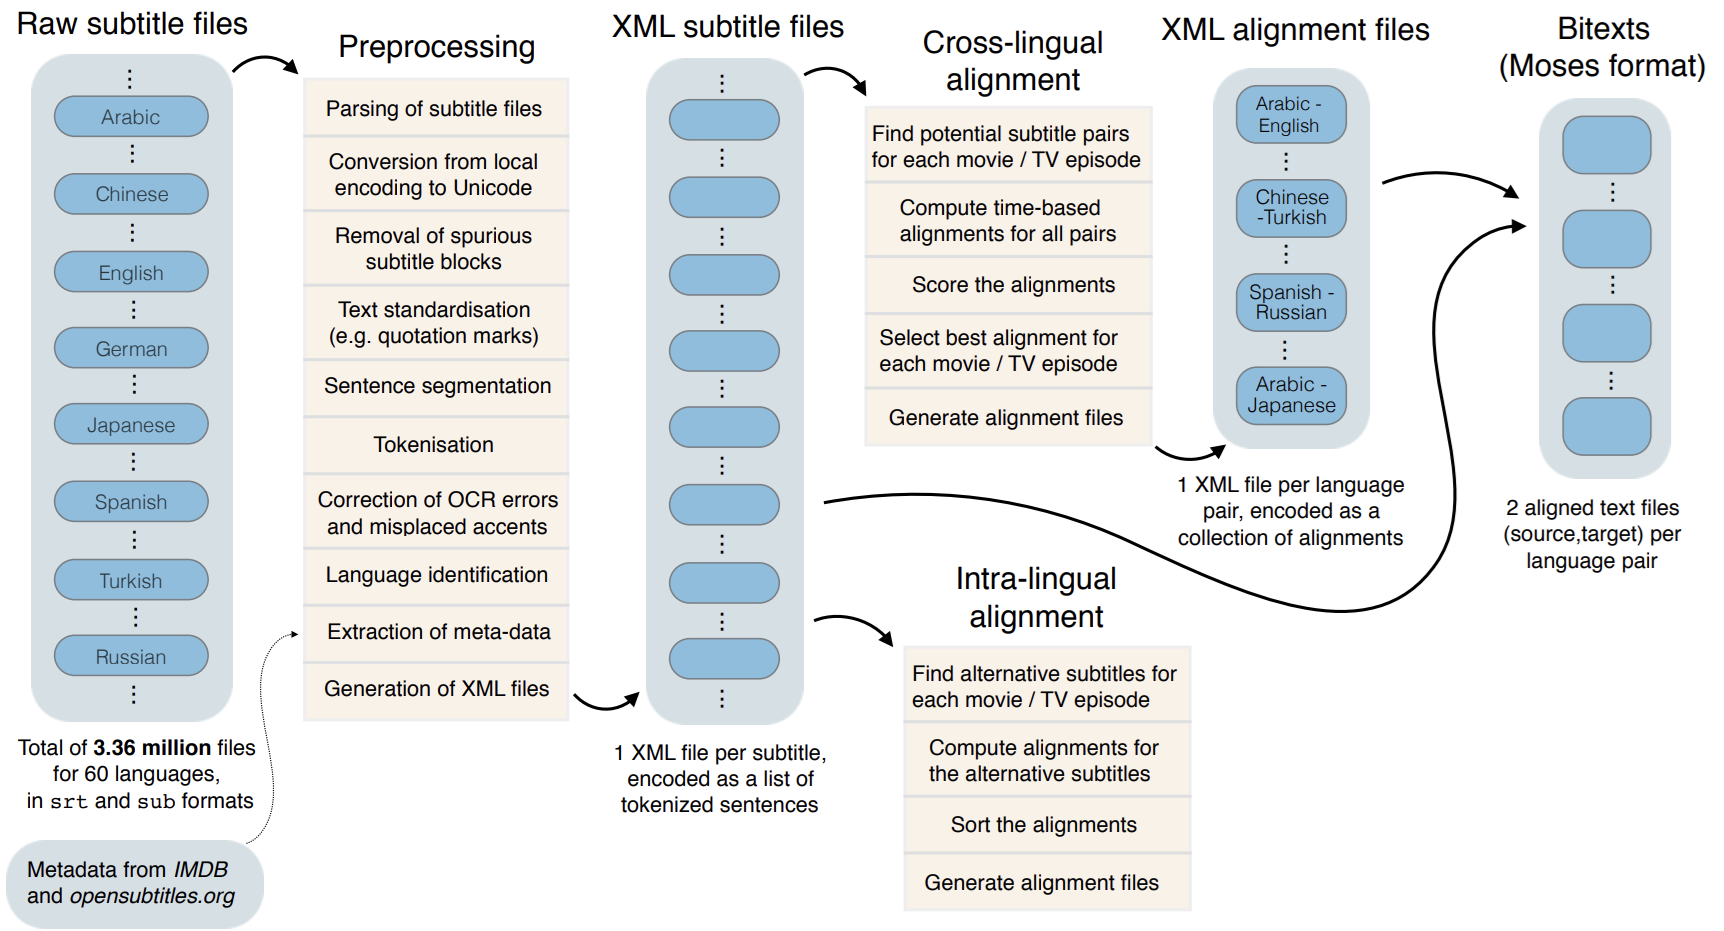
\includegraphics[width=\textwidth]{opensubs_corpus_processing.png}
	\caption{Pre-processing of the OPUS OpenSubtitles parallel corpus.}
	\label{fig:opensubtitles-pipeline}
\end{figure}

The OPUS Subtitles dataset contains not only the parallel sentences, but also movie identifiers from the Internet Movie Database (\textit{IMDB}) \footnote{\url{https://www.imdb.com/}}, which enables us to reconstruct the movie from whose script each sentence originates.
While the dataset contains contiguous subtitles, these are not appropriate input data for the NSP task, as film subtitles consist of dialogue instead of continuous text.
Our preliminary tests showed this, as our NSP model showed very low performance when given contiguous subtitle sentences pairs as inputs.

\subsection{Construction of NSP Corpora}
As mentioned in Section \ref{sec:document-level-corpus}, the next sentence prediction task requires consecutive sentences in order to be performed.
Out of the two context-specific corpus types which we employ, only Wikipedia articles consist of such consecutive sentences.
This is confirmed by the fact that preliminary investigations showed that the NSP model's performance on OpenSubtitles corpora was essentially equal to that of random guessing.
Thus, the NSP task is only performed on Wikipedia articles.
The NSP corpus of an article is constructed by simply taking each consecutive sentence pair from the article, constituting an input datum for the NSP model with an \texttt{is\_next} label of \texttt{True}.
We do not construct negative examples, for the reason that the most words with the most impact on the performance of the model would be words that tell the model that two sentences are \textit{not} connected, which does not appear to us to be useful information.

\subsection{Corpus Characteristics} \label{sec:corpus-characteristics}
We have described the sources of the corpora used in the implementation of our approach, but to gain a better understanding of the data, Table \ref{tbl:corpus-sizes} shows a few key metrics of each corpus type.
It can readily be seen that, while the corpora taken from the OpenSubtitles subtitles are composed of more lines on average, the Wikipedia articles feature much longer sentences (over three times longer on average than the sentences in subtitles).
This makes sense, as Wikipedia articles are written in an academic style, while movie subtitles tend to be more informal.
Wikipedia articles also contain a higher number of unique words on average, despite containing a lower number of words in total.
This may hint at a higher diversity of vocabulary employed in articles, although a higher number of named entities may also contribute to the higher count of unique words.

\begin{table}[ht]
	\centering
	\begin{tabular}{lrrrrr}
\toprule
 & Corpora & Avg. lines & Avg. words & Avg. unique words & Avg. words per line \\
Corpus Type &  &  &  &  &  \\
\midrule
Wikipedia article & 210 & 253 & 4382 & 1211 & 17.3 \\
OpenSubs subtitle & 632 & 901 & 5436 & 1050 & 6.0 \\
\bottomrule
\end{tabular}

	\caption{General statistics on corpora, per corpus type.}
	\label{tbl:corpus-sizes}
\end{table}


For a more granular overview, we also show these metrics for individual categories in Table \ref{tbl:corpus-sizes-per-wiki-category}.
Most obvious is the fact that the articles of World War II political leaders are, on average, much longer than those films or actors of either gender.
Another notable pattern is that the articles of male actors tend to be longer than those of their female counterparts.


\begin{table}[ht]
	\centering
	\begin{tabular}{lrrrrr}
\toprule
 & \# Corpora & Lines & Words & Unique Words & Words per Line \\
Wikipedia Category &  &  &  &  &  \\
\midrule
1980s English-language films & 26 & 160 & 2950 & 1014 & 18.4 \\
20th-century American actresses & 55 & 188 & 3296 & 934 & 17.5 \\
20th-century American male actors & 108 & 245 & 4157 & 1180 & 17.0 \\
World War II political leaders & 21 & 575 & 10159 & 2340 & 17.7 \\
\bottomrule
\end{tabular}

	\caption{General statistics on corpora, per Wikipedia article category.}
	\label{tbl:corpus-sizes-per-wiki-category}
\end{table}

\section{XAI Methods} \label{sec:xai-methods}
In order to appraise the influence of words in a corpus on the performance of an AI model performing NLP tasks on it, this work employs Explainable AI methods, as explained in Section \ref{sec:xai-as-tools-of-analysis}.
This section first puts forth the desiderata for the XAI methods, and then presents our choices of methods.
Due to time constraints, we limited our research to relatively simple methods.
While we gained valuable insights with the methods presented in this chapter, we acknowledge that better results may be achievable by using XAI approaches with more robust research.

\subsection{Desiderata}
Section \ref{sec:explainable-ai} has introduced essential distinctions between XAI methods which help us determine which methods are appropriate for our purpose:
We employ local, feature attribution methods of both model-specific and model-agnostic type, as these allow use to gauge the importance of words in the input from multiple points of view.
Model-specific methods have an advantage in terms of computational efficiency, as they generally require fewer model calls to attribute importances to features, instead leveraging the internal structure of a model to arrive at explanations.
On the other hand, model-agnostic methods are useful in that they can be used on any model and gauge the input-output relationship by performing actual experiments on the model, by observing the way changes to the model input change its output.

There is another desideratum which we impose on our XAI methods:
The XAI method should allow for processing the input sentences in its original form and not only as a \textit{bag of words}:
Some methods, such as SHAP \cite{lundbergUnifiedApproachInterpreting2017} and LIME \cite{ribeiroWhyShouldTrust2016}, were originally developed for structured data with a fixed number of input features.
When they are used on NLP tasks, they typically use as inputs not the textual data in its raw form, but rather vectors indicating whether a particular word is present in the sentence, with no regard to the word order and thus of syntactic relations between words.
In our view, this is problematic, as simplification of the input could lead the methods to attribute low importance to words such as "not", which only affect the meaning of a sentence in combination with its other words.
For this reason, we did not employ the popular XAI methods SHAP or LIME in this work.

In the following sections, we present three model-agnostic XAI methods which we use in the implementation of our vocabulary list generation approach described in Section \ref{sec:list-generation}.
These work by perturbing the inputs to the model and analyzing the changes in output.
The difference between them is how the perturbation is done:
Single Token Ablation removes single tokens from the inputs, whereas Single Token Summary works by setting the input to a single token.
The third method, Progressive Summary, attempts to find the most important words in sentences by iteratively building up the input sentence, one token at a time.
While the sections make reference to changes in "performance" to calculate word utility, this is only strictly accurate for the next sentence prediction task.
In the case of the sentence embedding task, we measure performance of the model on a permuted sentence by how close the output embedding vector is to the embedding of the unpermuted sentence, as explained in Section \ref{sec:sentence-embedding}.
After the model-agnostic methods, we detail our use of the model-specific transformer attention approach mentioned in Section \ref{sec:transformer}, as it requires more post-processing than the model-agnostic methods.

The relationship of the XAI methods to the NLP tasks is also discussed, as not every combination of XAI method and NLP task is feasible, either because it requires an unrealistic amount of computation or because the results of the combination are difficult to evaluate.
The results of the experiments with these methods is presented in Chapter \ref{ch:evaluation}.


\subsection{Single Token Ablation}
Our aim in using XAI methods is to find out which words, if known, improve the model's performance the most, when compared to not knowing the word.
Perhaps the simplest way of testing this is by going through every word in the AI model's input, and examining the impact on model performance when the word is removed from the input.
Within this work, this approach is called \textbf{Single Token Ablation}.
The processing steps performed in Single Token Ablation can be seen in Figure \ref{fig:single-token-ablation}.

\paragraph{Approach:}
For an input sentence, we run the model on the unmodified sentence to get a baseline performance.
We then get the unique words in the input by using the tokenizer and merging sub-word tokens back into words.
For each word in the input, we create a variation of the input where the word is removed.
We then run the model on all variations and measure the performance.
The estimated utility in this approach is then calculated by taking the difference in performance between the variation's performance and that of the baseline output.

\paragraph{Critical Evaluation:}
One advantage of Single Token Ablation is its conceptual simplicity, as it is easy to implement.
Furthermore, its time complexity is fairly low for a feature method, as it requires only one model call for each unique token in the sentence ($\mathcal{O}(n)$).
Before running experiments, we anticipated that due to this simplicity, Single Token Ablation would not work well on long sentences, where leaving out a single token would not seem to have a great impact on the meaning of the sentence.
Furthermore, this method does not take into account the utility of a word in the context of word combinations.
However, among the methods used in this paper, this method achieves the best results in the final evaluation.

\begin{figure}[H]
	\begin{center}
\scalebox{0.75}{
\begin{tikzpicture}[node distance=1.8cm and 2.5cm, every node/.style={font=\small}]

	% Styles
	\tikzstyle{process} = [rectangle, rounded corners, minimum width=3.5cm, minimum height=1cm, text centered, draw=black, fill=blue!10, text width=8.5cm]
	\tikzstyle{arrow} = [thick, ->, >=Stealth]
	\tikzstyle{data} = [align=left, text width=8.5cm, anchor=west]

	% Process Nodes
	\node (n1) [process] {Input sentence};
	\node (n2) [process, below=of n1] {Tokenize};
	\node (n3) [process, below=of n2] {Merge tokens, filter named entities and special tokens};
	\node (n4) [process, below=of n3] {Make sentence variations by ablating merged tokens};
	\node (n5) [process, below=of n4] {Run model for variations, evaluate performances};
	\node (n6) [process, below=of n5] {Calculate difference to baseline in performance};

	% Anchor point to align all data nodes horizontally
	\node (anchor) [right=of n1] {};

	% Data Nodes, all vertically stacked but aligned to 'anchor'
	\node (d1) [data] at (anchor) {"Abraham Lincoln faced enmity in 1863."};
	\node (d2) [data, right=of n2] {
['[CLS]', 'abraham', 'lincoln', 'faced', 'en', '\#\#mity', 'in', '1863', '.', '[SEP]']
};
	\node (d3) [data, right=of n3] { ['faced', 'enmity', 'in'] };
	\node (d4) [data, right=of n4] {
\textbf{Baseline:} "abraham lincoln faced enmity in 1863."\\
\textbf{faced:} "abraham lincoln enmity in 1863."\\
\textbf{enmity:} "abraham lincoln faced in 1863."\\
\textbf{in:} "abraham lincoln faced enmity 1863."\\
	};
	\node (d5) [data, right=of n5] {
\textbf{Baseline:} 0.8\\
\textbf{faced:} 0.5\\
\textbf{enmity:} 0.3\\
\textbf{in:} 0.7\\
	};
	\node (d6) [data, right=of n6] {
[('faced', 0.3), ('enmity', 0.5), ('in', 0.1)]
	};

	% Arrows between process nodes (left column)
	\draw [arrow] (n1) -- (n2);
	\draw [arrow] (n2) -- (n3);
	\draw [arrow] (n3) -- (n4);
	\draw [arrow] (n4) -- (n5);
	\draw [arrow] (n5) -- (n6);

\end{tikzpicture}
}
\end{center}

	\caption{Example of Single Token Ablation, on one sentence.}
	\label{fig:single-token-ablation}
\end{figure}

\subsection{Single Token Summary}
The second feature model-agnostic method can be seen as the opposite of Single Token Ablation:
Instead of taking out one word at a time, we use as input only a single word at a time.
Because the intention behind this method is finding words which, on their own, carry much of the meaning of a sentence, we call it \textbf{Single Token Summary}.

\paragraph{Approach:}
We first run the model on a variation of the input sentence where only punctuation and named entities are included, using the output as the starting performance.
We then decompose the input sentence into its word tokens.
For each word, a variation of the sentence is put through the model where, in addition with punctuation and named entities, only that word appears.
The utility in this approach is calculated by taking the performance improvement of a word's sentence variation compared to the starting performance.

\paragraph{Critical Evaluation:}
Like Single Token Ablation, this method requires only one model call for each unique token in the sentence ($\mathcal{O}(n)$).
This method may find tokens helpful to beginners more efficiently, however, as it simulates knowing only one word, whereas Single Token Ablation tests performance while taking into account the meaning of the other words in each sentence, as well.
However, this could the method to assign low utility to words which mostly convey meaning when in combination with other words, such as "not".

% \paragraph{Compatibility with NLP tasks:}
% \todo{compat with NSP?}

\subsection{Progressive Summary}
While Single Token Summary is easy to implement and computationally inexpensive, it has the conceptual disadvantage of not taking into account the utility of word combinations.
To achieve a more accurate evaluation, we present another "summary" approach, where the sentence is built up one word at a time.
We call this approach "Progressive Summary".

\paragraph{Approach:}
For an input sentence, this approach starts the same as Single Token Summary, by checking the performance of the one-word sentence variations.
We then rank the words by their performance improvements, and use the word with the highest improvement in the next iteration.
From the remaining words in the sentence, we check which one improves the performance the most when used in addition to our already found word.
By iterating this method, we progressively reconstruct the original sentence, which each step adding the word which improves the performance the most.
Here, the estimated utility of a word is the boost in performance which is brought to the sentence when the word is added.

\paragraph{Critical Evaluation:}
For a single sentence, Progressive Summary would appear to be the most accurate in ordering its words by utility, as it considers the utility of each word in combination with the words which have already been found to be useful.
However, Progressive Summary is much more computationally intensive than Single Token Summary, which requires only one model call per word in the sentence.
Because of its iterative approach, for a sentence with 10 words, Progressive Summary calls the model $10+9+8+... = \sum_{i=1}^{n}i = \frac{n^2 + n}{2}$ times, which is a time complexity of $\mathcal{O}(n^2)$.

\paragraph{Compatibility with NLP tasks:}
As Progressive Summary starts from a set of one words and then progresses to larger sets, we do not consider it appropriate to employ in combination with next sentence prediction.
One could circumvent the issue by leaving one of the sentences in its original form and only perturbing the other, but this can hardly be seen as a modeling of natural language ability.
As such, our implementation does not use Progressive Summary with next sentence prediction.

\paragraph{Summary:}
Progressive Summary attempts to find the most important words in a sentence one by one, by first reducing the sentence to one word, then two etc., and using a distance metric to compare the "summaries" to the original sentence.
The words which bring the model output for the summary closest to that of the original sentence are regarded as the most useful.

\subsection{Attention as Explanation}
The model-agnostic methods so far could be employed on any AI model.
However, as many of the latest state-of-the-art AI models follow the Neural Network architecture, and more specifically the transformer architecture (see Section \ref{sec:transformer}), we also attempt word utility estimation with method specific to these models, namely attention.
% These model-specific XAI methods have the advantage of being computationally efficient:
% Model-agnostic methods extract information about the model by perturbing its inputs and analyzing the resulting changes in the output.
% This requires many model calls for one input datum.
% In contrast, model-specific methods can analyze the input-output relationship with only one model call, as they look into the model itself for information.
% We therefore try two model-specific methods for analyzing word utility as well, as their more efficient calculations means they can process more input data in a given time, which should increase the accuracy of the resulting word list for large corpora.
As stated before, transformer models use self-attention to assign importance to the connections between tokens in the input (if their input is in text format).
This may be used as a kind of explanation, as words which have strong connections to many other words in the sentence presumably are more important to the AI model's understanding of it than those receiving less self-attention.

An important difference to the model-agnostic methods explained before is that we do not control word masking with a tokenizer \textit{independent of the model}, thus the splitting of words is not under our direct control.
The tokenizers used are \texttt{bert-base-uncased} and \texttt{sentence-transformers/paraphrase-MiniLM-L6-v2}.
These produce tokens on a sub-word level, which means that we must perform post-processing on the attentions to acquire values on the word level and make vocabulary lists than contain full words.
For BERT tokens, this is a simple process as sub-tokens which are not at the beginning of a word start with "\#\#" (See Section \ref{sec:tokenization}).
The estimated utility for the reconstructed token is calculated by taking the sum of the attention values of each sub-token.

\paragraph{Approach:}
A transformer model is run with one line as input.
The transformer outputs an attention tensor, which attributes a value to each pair of tokens in the input (this includes special tokens from the tokenizer, such as \texttt{[SEP]}, and punctuation).
We then aggregate the attention of each token by summing over one axis of the attention tensor of all connections each token has, and over all the attention heads, resulting in one scalar value per token.
The original tokens of the tokenizer are merged
Next, special tokens and punctuation are filtered
Finally, we normalize the attentions such that the attention for all words in the line sums up to one.
The attributed attention to a word is its estimated utility.

\paragraph{Critical Evaluation:}
As hinted at before, this method uses one model call for one input line, and thus has a time complexity of $\mathcal{O}(1)$.
One disadvantage of attention as our explanation mechanism is that attentions are attributed to input tokens of the model.
Unlike the model-agnostic methods where word masking is controlled by a tokenizer \textit{independent of the model}, the tokenizer cannot be changed.
AI models are trained with some tokenizer as preprocessing the input, and this tokenizer cannot be changed, lest we change the input format to the AI model itself.
This is an issue because it means that lists generated with the model-specific tokenizer are not necessarily comparable to lists from model-agnostic methods, as the tokenization method may differ.
In addition to this technical downside, attention is controversial as a mechanism to explain model decisions:
One point of critique is that, while attention influences the model's behavior, it is not a faithful explanation because alternative attention distributions can yield similar model outputs \cite{jainAttentionNotExplanation2019}.
On the other hand, it has been argued that the mere fact that a model chooses a particular attention distribution, rather than another, means that the actually generated distribution is a more plausible explanation that artificial adversarial distributions \cite{wiegreffeAttentionNotNot2019}.
As we will show in our list evaluation, when used with our list generation approach, attention produces vocabulary lists that are close in efficiency to those produced by the model-agnostic methods.

\paragraph{Summary:}
Among the XAI methods used in this work, Attention as Explanation requires the least resources, and it is not restricted to any one NLP task (although the model must be of transformer type).
However, we do not control the tokenizer used directly.
While the NSP model uses the same tokenizer that is also used for token masking in the model-agnostic XAI methods, the sentences embedding model uses a different tokenizer.



% \subsubsection{Layer-wise Relevance Propagation (not yet implemented $\rightarrow$ may be deleted)}
% \paragraph{Approach:}
% \paragraph{Advantages:}
% \paragraph{Disadvantages:}
% \paragraph{Summary:}
%
%
\section{Implementation with Chosen NLP Tasks, Corpora, and XAI Methods} \label{sec:implementation-final}
The previous chapters have argued for the choice of components in our theoretical approach to vocabulary list generation and evaluation.
This final section about our implementation describes how the chosen components interact in our implementation.

\todo{ Describe which comps are compatible, and where it is not obvious, how exactly they are made to work with each other. }

\begin{figure}[H]
	\begin{center}
	\scalebox{0.75}{
		\begin{tikzpicture}[node distance=1.8cm and 2.5cm, every node/.style={font=\small}]

			% Styles
			\tikzstyle{process} = [rectangle, rounded corners, minimum width=3.5cm, minimum height=1cm, text centered, draw=black, fill=blue!10, text width=8.5cm]
			\tikzstyle{arrow} = [thick, ->, >=Stealth]
			\tikzstyle{data} = [align=left, text width=8.5cm, anchor=west]

			% Process Nodes
			\node (n1) [process] {Input sentence};
			\node (n2) [process, below=of n1] {Tokenize};
			\node (n3) [process, below=of n2] {Merge tokens, filter named entities and special tokens};
			\node (n4) [process, below=of n3] {Make sentence variations by ablating merged tokens};
			\node (n5) [process, below=of n4] {Run model for variations, evaluate performances};
			\node (n6) [process, below=of n5] {Calculate difference to baseline in performance};

			% Anchor point to align all data nodes horizontally
			\node (anchor) [right=of n1] {};

			% Data Nodes, all vertically stacked but aligned to 'anchor'
			\node (d1) [data] at (anchor) {\textbf{Baseline}: "Abraham Lincoln faced enmity in 1863."\\
				\textbf{Variation}: "Abraham Lincoln enmity 1863."
			};
			\node (d2) [data, right=of n2] {
			['[CLS]', 'abraham', 'lincoln', 'faced', 'en', '\#\#mity', 'in', '1863', '.', '[SEP]']
			};
			\node (d3) [data, right=of n3] { ['faced', 'enmity', 'in'] };
			\node (d4) [data, right=of n4] {
				\textbf{Baseline:} "abraham lincoln faced enmity in 1863."\\
				\textbf{faced:} "abraham lincoln enmity in 1863."\\
				\textbf{enmity:} "abraham lincoln faced in 1863."\\
				\textbf{in:} "abraham lincoln faced enmity 1863."\\
			};
			\node (d5) [data, right=of n5] {
				\textbf{Baseline:} 0.8\\
				\textbf{faced:} 0.5\\
				\textbf{enmity:} 0.3\\
				\textbf{in:} 0.7\\
			};
			\node (d6) [data, right=of n6] {
				[('faced', 0.3), ('enmity', 0.5), ('in', 0.1)]
			};

			% Arrows between process nodes (left column)
			\draw [arrow] (n1) -- (n2);
			\draw [arrow] (n2) -- (n3);
			\draw [arrow] (n3) -- (n4);
			\draw [arrow] (n4) -- (n5);
			\draw [arrow] (n5) -- (n6);

		\end{tikzpicture}
	}
\end{center}


	\caption{Example of sentence embedding scoring}
	\label{fig:list-evaluation-diagram}
\end{figure}

\subsection{Supported Languages}
Our data pipeline contains various language-specific components, all of which must support a language in order for our approach to support vocabulary list generation in the language.
Table \ref{table:supported-languages} summarizes the language support of each component, including pre-processing.

	{
		\renewcommand{\arraystretch}{1.5}  % Increase the vertical padding for this table only
		\begin{table}[H]
			\centering
			\begin{tabularx}{\textwidth}{|X|X|X|}
				\hline
				\textbf{Component}                          & \textbf{Supported Languages} & \textbf{Notes}                                                                                                                                                                                                                             \\
				\hline
				Tokenization                                & 104                          & Using the \texttt{bert-base-uncased} model\footnotemark[1]                                                                                                                                                                                 \\
				\hline
				Named Entity Recognition                    & 9                            & Using the \textit{spacy} model \texttt{xx\_ent\_wiki\_sm}\footnotemark[2]. The number of supported languages is not stated for this model, but it was trained on the \texttt{WikiNER} dataset\footnotemark[3], which contains 9 languages. \\
				\hline
				Next sentence prediction                    & 104                          & Using the \texttt{bert-base-multilingual-cased} model\footnotemark[4]                                                                                                                                                                      \\
				\hline
				Sentence Embedding                          & $>50$                        & Using the \texttt{paraphrase-multilingual-MiniLM-L12-v2} model\footnotemark[5]                                                                                                                                                             \\
				\hline
				Sentence splitting (for Wikipedia articles) & $>150$                       & Using the \texttt{xx\_sent\_ud\_sm} model\footnotemark[6], based on the \textit{Universal Dependencies} framework\footnotemark[7], which supports $>150$ languages.                                                                        \\
				\hline
				Filtering of Wikipedia sections             & (manual)                     & See Section \ref{sec:wikipedia-preprocessing}                                                                                                                                                                                              \\
				\hline
				Wikipedia Corpus                            & $>300$                       & As of 2025, there exist Wikipedias in over 300 languages\footnotemark[8]                                                                                                                                                                   \\
				\hline
				OPUS OpenSubtitles Corpus                   & 94                           & See \footnotemark[9]                                                                                                                                                                                                             \\
				\hline
			\end{tabularx}



			\caption{Languages supported by each component in the pipeline.}
			\label{table:supported-languages}
		\end{table}
	}

\footnotetext[1]{\url{https://huggingface.co/google-bert/bert-base-uncased}}
\footnotetext[2]{\url{https://spacy.io/models/xx\#xx_ent_wiki_sm}}
\footnotetext[3]{\url{https://huggingface.co/datasets/mnaguib/WikiNER}}
\footnotetext[4]{\url{https://huggingface.co/google-bert/bert-base-multilingual-cased}}
\footnotetext[5]{\url{https://www.sbert.net/docs/sentence_transformer/pretrained_models.html\#original-models}}
\footnotetext[6]{\url{https://spacy.io/models/xx\#xx_sent_ud_sm}}
\footnotetext[7]{\url{https://universaldependencies.org/}}
\footnotetext[8]{\url{https://en.wikipedia.org/wiki/List_of_Wikipedias}}
\footnotetext[9]{\url{https://opus.nlpl.eu/OpenSubtitles/corpus/version/OpenSubtitles}}

It can be seen that, apart from the manual selection of certain Wikipedia headings, named entity recognition is the bottleneck in our pipeline with the currently used packages. 
While we did not individually cross-correlate the supported languages of each component, we estimate that the pipeline supports 9 languages when taking into consideration the \textit{spacy} NER capabilities.
With a NER model supporting more languages, the implementation is estimated to support at least 40 languages, as the next bottleneck would be the sentence embedding model with over $50$ languages, some of which may, however, not be supported by all other components.
	
	
	
